\subsection{Основні означення теорії графів}

Введемо деякі означення з теорії графів, які є необхідними для розуміння теорем і означень зі спектральної теорії.

 %%визначення графа. 
 \textbf{Означення 1.}\\ 
 \textit{Графом} $G =(V,E)$ називається така пара впорядкованих множин $V$ і $E$,  де $V$ --- множина вершин, що є непорожньою і скінченною, а $E$ --- множина ребер, що складається з невпорядкованих пар елементів множини вершин.
 
Введемо такі позначення, які надалі будемо використовувати у роботі:\\
-- $E(G)$ --- множина ребер $E$ графа $G$.\\
-- $V(G)$ --- множина вершин $V$ графа $G$.\\
-- $(u,v)$ --- ребро, що з'єднує вершини $u$ і $v$.\\
Такі уточнення допомагають розуміти про ребра та вершини, якого графа йшлося.

\textbf{Приклад 1.}
\begin{figure}[H]
    \centering
    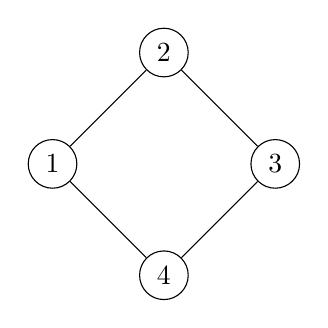
\begin{tikzpicture}[node distance={20mm}, main/.style = {draw, circle}]
    \node[main] (1) {$1$}; 
    \node[main] (2)[above right of=1] {$2$};
    \node[main] (3)[below right of=2] {$3$};
    \node[main] (4)[below left of=3] {$4$};
    \draw (1) -- (2);
    \draw (2) -- (3);
    \draw (3) -- (4);
    \draw (4) -- (1);
    \end{tikzpicture}\\
    \caption{G}
    \label{ris1:image}
\end{figure}
Знайдемо чому дорівнюють множина вершин і ребер графа $G$, який зображено на рисунку \ref{ris1:image}. Вершини --- точки, що позначені на площині, тобто $V(G) = \{1,2,3,4\}$,  а ребра --- це лінії, що їх з'єднують, тобто  $V(G) = \{(1,2),\ (2,3),\ (3,4),\ (4,1)\}$.



%% Реберно зважений граф
 \vskip 1pt  
 \textbf{Означення 2.}\\
  {\itРеберно-зваженим графом $\bf G$} називається така пара $(G, w)$, де $G$ --- це граф, а $w: E\rightarrow (0, +\infty)$ --- вагова функція, відображення множини $E(G)$ на множину додатніх дійсних чисел.
 
  Вагу $w(e)$ ребра $e$, будемо позначати $w_e$. Також надалі замість терміну ``реберно-зважений граф'' будемо писати ``зважений граф'', оскільки це більш зручно і така назва також зустрічається у літературі і вважається загальноприйнятим. 
  
\textbf{Приклад 2.}
 \begin{figure}[H]{}
    \centering
    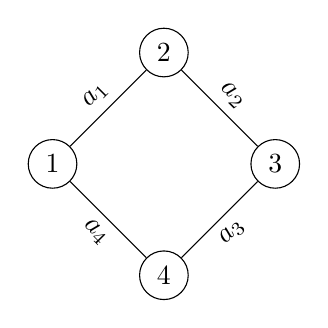
\begin{tikzpicture}[node distance={20mm}, main/.style = {draw, circle}]
    \node[main] (1) {$1$}; 
    \node[main] (2)[above right of=1] {$2$};
    \node[main] (3)[below right of=2] {$3$};
    \node[main] (4)[below left of=3] {$4$};
    \draw (1) -- node [midway, above, sloped] {$a_1$}(2);
    \draw (2) -- node [midway, above, sloped] {$a_2$}(3);
    \draw (3) -- node [midway, below, sloped] {$a_3$}(4);
    \draw (4) -- node [midway, below, sloped] {$a_4$}(1);
    \end{tikzpicture}\\
    \caption{Реберно-зважений граф \textbf{G}}
    \label{ris2:image}
\end{figure}

На рисунку \ref{ris2:image} зображений зважений граф \textbf{G}, що має 4 вершини і 4 ребра. Випишемо вагу для кожного ребра: $(1,2):w_{12} = a_1$,  $(2,3):w_{23} = a_2$,  $(3,4):w_{34} = a_3$,  $(4,1):w_{41} = a_4$.

%% Суміжність, інцидентність, матриця суміжності

 \textbf{Означення 3.}\\
 \emph{Суміжні} вершини --- це вершини графа, що з’єднані ребром.
  
  \textbf{Означення 4.}\\
  Вершину $u$ і ребро $e$ називають \emph{інцидентними}, якщо $e = (u,v)$, тобто вершина $u$ є кінцем ребра $e$.
 
  \textbf{Означення 5.}\\
\textit{Степінь вершини $\deg v$} --- це кількість ребер, що інцидентні вершині $v$.
 
\textbf{Приклад 3.}\\
Знайдемо степінь, інцидентні ребра і суміжні вершини для першої вершини графа $G$ (див. рисунок \ref{ris1:image}).
Оскільки вершини  $1$ і $2$, та $1$ і $4$ з'єднані ребром, то вони є суміжними. Отже, інцидентними ребрами до вершини 1 будуть ребра $(1,2)$ і $(1,4)$ і степінь вершини буде дорівнювати 2.

У книгах [8]-[10] можна дізнатись більше деталей з загальної теорії графів.